\documentclass[11pt]{article}
\usepackage[T1]{fontenc}
\usepackage{lmodern}
\usepackage[margin=0.9in]{geometry}
\usepackage{amsmath,amssymb,amsthm}
\usepackage{graphicx}
\usepackage{booktabs}
\usepackage[font=small,labelfont=bf]{caption}
\usepackage[hidelinks]{hyperref}
\usepackage{enumitem}
\usepackage{float}
\usepackage{multicol}
\graphicspath{{../figures/}}
\newcommand{\repourl}{github.com/djangothompson12-alt/Fortnite-Token-Probability-}

\theoremstyle{definition}
\newtheorem{definition}{Definition}[section]
\newtheorem{remark}[definition]{Remark}
\theoremstyle{plain}
\newtheorem{proposition}[definition]{Proposition}

\title{\textbf{Token or True Love?}\\[4pt] \large A statistical analysis of whether you are more likely to find the Fortnite Pirate Shop Token or be wifed up for Christmas}
\author{Django Thompson\\[2pt] \small Preprint DOI: \href{https://doi.org/10.5281/zenodo.24150193}{\texttt{10.5281/zenodo.24150193}}\\ \small Code and data: \texttt{\repourl}}
\date{12 November 2026}

\raggedbottom
\begin{document}
\maketitle

\begin{abstract}
\noindent
Two seemingly impossible tasks: which one is more likely? The first is finding Fortnite's Pirate Shop Token, which drops from 1 in 137{,}500 chests and makes everything in the Item Shop that costs V-Bucks free for 14 days; the second is getting a girlfriend, which has no published drop rate at all. I model the token as a thinned Poisson process shaped by how long a player survives and how quickly matchmaking catches up with him, and the girlfriend as a Drake-style chain of filters calibrated to US survey data, adjusted for looks, personality, effort and (last but not least) height. A solo player needs a median of about 3{,}240 hours to find the token. A squad needs 1{,}250, because the token is shared. For a man who is looking and plays 10 hours a week, a girlfriend is three times as likely before the season ends on 5 December. The token pulls ahead only past roughly 23 hours a week, by which point he has stopped leaving the house, and height moves that line from 20 hours at 5'5'' to 30 at 6'3''. Fortunately, Fortnite skill barely matters, but dying off spawn does. Using Epic's own player counts, I estimate that about 14{,}000 tokens are found every day and that nobody you know has one.
\end{abstract}

\noindent{\small\textit{Disclaimer.} Fortnite is a trademark of Epic Games, Inc. Portions of the materials used are trademarks and/or copyrighted works of Epic Games, Inc. All rights reserved by Epic. This material is not official and is not endorsed by Epic. AI was used to help code and run simulations for this project.}

\section{Preliminaries}

Epic confirmed the drop rate in early November 2026~\cite{status,vgc}. Before that, the internet had settled on 1 in 700{,}000~\cite{timesaver}, so the real odds turned out five times better than feared, which moves the token from impossible to merely pointless.

\begin{definition}[The Token]
A \emph{chest} is a Bernoulli trial with success probability $p = 1/137{,}500$. A success in any chest opened by any member of a group is credited to every member still in the match~\cite{gamesradar}. (This last clause turns out to matter. See Remark~\ref{rem:tg}.)
\end{definition}

\begin{definition}[The Girlfriend]
A \emph{girlfriend} is a relationship that forms before a stated deadline. I take the deadline to be 5 December, when the season ends (just in time for ``cuffing'' season).
\end{definition}

I borrow the girlfriend side from Backus~\cite{backus}, who used the Drake equation to explain why he was single. Economists treat the same problem as search with friction, such as looking for a job or a house~\cite{mortensen}. For simplicity, mine is the most basic version of both: people met, multiplied by the chance each one works out.

\paragraph{Related work.} As far as I can find, nobody has raced a drop rate against a love life. Each half has its own literature, though. Rare loot is more arousing than common loot and makes players want to open more~\cite{larche}. Players hold badly wrong folk models of drop odds even when the odds are published~\cite{wen,xiao}, and showing people only the winners inflates their belief that they will win too~\cite{cordes}, which is more or less what a viral ``I found the token'' clip does. On the other side, online dating messages flow up a steep ladder of desirability and replies thin out the higher you aim~\cite{bruch}. Whether gaming crowds out offline social life is still disputed~\cite{kowert,domahidi}. Optimal stopping asks when to stop looking~\cite{chow}, and its two-sided version, with everyone searching at once, is closer to real dating~\cite{eriksson}.

\section{The Token Process}

Let $\bar T_n$ be a player's mean survival time in match $n$. Skill-based matchmaking (SBMM) pulls it down from $T_0 = 14$ minutes towards a personal floor $T^\infty_j$,
\begin{equation}
\bar T_{n} = (1-\phi)^{k}\big[T^\infty_j + (T_0 - T^\infty_j)e^{-n/\tau}\big], \qquad T^\infty_j = 6\,e^{0.35 z_j},
\end{equation}
where $z_j$ is the player's skill in standard deviations and $(1-\phi)^k$ is fatigue, 1\% per game into a session. That is generous: in League of Legends, performance drops by more than 10\% across a session~\cite{sapienza}. Chests per match are Poisson with mean
\begin{equation}
\mathbb{E}[c_n] = \sigma C\big(1 - e^{-T_n/\kappa}\big), \qquad C = 12,\ \kappa = 6 \text{ min},
\end{equation}
because most chests are opened soon after landing. Here $\sigma$ is the share of chests you open yourself (1 solo, 0.65 in a squad). Every match also costs about 4 minutes of lobby, queue, Battle Bus and skydive. Survival time $T$ is counted from the moment you land, not from when the bus sets off. Everything before you land is in those 4 minutes.

\begin{proposition}[Charnov's rule with an exponential loot curve]
Ignoring fatigue and noise, chests per hour $r(T) = 60C(1 - e^{-T/\kappa})/(T + O)$, with $O$ the time between matches, is maximised at
\[
T^* = -\kappa\big[W_{-1}(-e^{-(1+O/\kappa)}) + 1\big] - O,
\]
where $W_{-1}$ is the lower branch of the Lambert $W$ function.
\end{proposition}

\begin{proof}
$r'(T)=0$ gives $e^{T/\kappa} = 1 + (T+O)/\kappa$. Put $x = 1 + (T+O)/\kappa$ to get $-xe^{-x} = -e^{-(1+O/\kappa)}$. The principal branch gives $T<-O$, so $x = -W_{-1}(-e^{-(1+O/\kappa)})$.
\end{proof}

This is the marginal value theorem from foraging ecology~\cite{charnov}. A bird should leave a bush once it is eating slower than its average for the whole trip; a player should leave a match once he is looting slower than his average including the time before the game (lobby and landing). Foraging papers already have the Lambert $W$ form. I only supply the Fortnite numbers: with $O = 4$ and $\kappa = 6$, $T^* = 5.82$ minutes, or \textbf{5 minutes 49 seconds} after landing. On the in-game clock that is roughly 7 minutes after the bus leaves, since the bus ride and the drop take about a minute and a half, depending on when you jump. There is no mathematical reason for your character to be alive after that. You most likely won't win, and battle royale results are mostly luck anyway~\cite{rosenbusch}, so leaving the game is the best option. People in foraging experiments tend to overstay too~\cite{saravanakumar}, which describes every player who has ever chased a Victory Royale.

\begin{remark}[Typical Gamer]\label{rem:tg}
The rule does not survive contact with squads. The YouTuber Typical Gamer spent about 80 hours hunting the token, left a squad match as a joke, and watched his teammates find it moments later~\cite{dexerto}. The model gives a squad about a 4.5\% chance of a find within 80 hours. So only leave at 5:49 if your whole squad leaves with you.
\end{remark}

\paragraph{Skill.} The job is opening chests, not winning. So skill should matter less than people assume, and the model agrees (Table~\ref{tab:token}, right): because $r(T)$ is nearly flat around $T^*$, anyone who survives somewhere between 4 and 9 minutes on average loots within 6\% of the best possible rate. Dying off spawn is the real penalty. It costs 37\% more hours. Oddly, being very good costs you too, since a top-1\% player stays alive so long that he needs 18\% more hours than the median player. So even good players should leave early.

\begin{table}[!htbp]
\centering\small
\caption{Left: hours of play to find the token by mode (10th, 50th and 90th percentiles of players). Right: median solo hours by skill, scaled to the full model's median.}
\label{tab:token}
\begin{tabular}[t]{lrrr}
\toprule
Mode & Lucky 10\% & Median & Unlucky 10\% \\
\midrule
Solo  & 480 & 3{,}244 & 10{,}800 \\
Duo   & 279 & 1{,}902 & 6{,}339 \\
Squad & 180 & 1{,}246 & 4{,}136 \\
\bottomrule
\end{tabular}
\qquad
\begin{tabular}[t]{lrr}
\toprule
Skill & Survival & Median \\
\midrule
Dies off spawn & 2.0 min & 4{,}430 \\
Bottom 10\% & 3.8 min & 3{,}440 \\
Median & 6.0 min & 3{,}244 \\
Top 10\% & 9.4 min & 3{,}410 \\
Top 1\% & 13.5 min & 3{,}830 \\
\bottomrule
\end{tabular}
\end{table}

The median of 3{,}244 hours is 135 days without sleep. Once SBMM catches up, matches get so short that 40 to 65\% of the time spent ``playing Fortnite'' is spent in the lobby.

\section{The Partner Process}

\begin{definition}[Backus chain]
Each new person met is a trial with success probability
\[
\pi = \underbrace{0.5}_{\text{woman}}\cdot\underbrace{0.4}_{\text{age}}\cdot\underbrace{0.34}_{\text{single}}\cdot\underbrace{0.35}_{\text{looking}}\cdot\underbrace{\tfrac{1}{20}}_{\text{attracted}}\cdot\underbrace{\tfrac{1}{10}}_{\text{get on}}\cdot\underbrace{0.5}_{\text{you ask}}\cdot\underbrace{0.5}_{\text{she says yes}} \approx \frac{1}{33{,}600}.
\]
The attraction and compatibility filters follow Backus~\cite{backus}; the single and looking shares are from Pew~\cite{pew23}.
\end{definition}

He meets about one new person a day, minus whatever socialising Fortnite has replaced. Men his age average 0.51 hours a day socialising and 1.08 hours gaming~\cite{atus}. Gaming is already winning. A cold DM gets a reply 8\% of the time (my guess), and the reply then has to survive a conversation, a date and actually becoming a thing, which works out at about 1 in 3{,}500. That is 40 times better than a chest, per try. The chest wins on volume, at about 30 an hour.

Only half of single men are looking~\cite{pew23}, so half the simulated men are, and the rest stumble into something at a fifth of the rate. Each man gets a looks percentile (worth up to an 11-fold gap online~\cite{okc}), a lognormal personality factor, and an effort multiplier of 1, 2.5 or 5 (casual, active, all out; I made these up). Apps are in the model, with a measured 0.6\% match rate for men~\cite{tyson}, but the headline numbers are for men not on them~\cite{pewod}.

I then tune two unknowns until the model reproduces two real numbers: 63\% of men aged 18--29 are single~\cite{pew23}, and 39\% of couples who got together in 2017 met online~\cite{hcmst}. Taken literally, Backus's chain leaves the average man waiting 63 years. Calibrated, the wait is about two. Real life is roughly 30 times kinder than meeting strangers, presumably because most people end up with someone they already know.

\begin{definition}[Height factor]
Let $h$ be height in cm. US men aged 20--29 average 176.3 cm (5'9.4''), with 5th and 95th percentiles of 162.0 and 188.1 cm~\cite{nhanes}, so $\mathrm{sd}(h) \approx 7.9$ cm. Men 6'3''--6'4'' receive 65\% more first messages online than men 5'7''--5'8''~\cite{hitsch}. That gives a log-slope of $\beta = 0.0246$ per cm, which I apply to the whole funnel:
\[
\lambda_j \;\mapsto\; \lambda_j\, e^{\beta(\min(h_j,\,188) - 176.3)}.
\]
The cap reflects the finding that the advantage levels off above six feet~\cite{hensley}.
\end{definition}

This is an upper bound. First messages are not relationships, and a conjoint study that holds looks fixed finds that height, like job, bio and intelligence, has an effect 7 to 20 times smaller than attractiveness~\cite{witmer}. Table~\ref{tab:height} also shows the result with $\beta$ halved. Average height gives a multiplier of 1, so no changes to earlier results.

\begin{table}[!htbp]
\centering\small
\caption{Height. Chance of a girlfriend by Christmas for an average man actively trying (10 h/week, no apps), and the weekly hours at which the token overtakes (solo, casually looking).}
\label{tab:height}
\begin{tabular}{lrrrrr}
\toprule
Height & Percentile & Multiplier & By Christmas & ($\beta/2$) & Crossover \\
\midrule
5'5'' & 8th & 0.76 & 6.5\% & 7.4\% & 20 h/wk \\
5'7'' & 22nd & 0.86 & 7.4\% & 7.9\% & 22 h/wk \\
5'9'' & 45th & 0.98 & 8.3\% & 8.4\% & 24 h/wk \\
5'11'' & 69th & 1.10 & 9.3\% & 8.9\% & 26 h/wk \\
6'1'' & 87th & 1.25 & 10.5\% & 9.5\% & 28 h/wk \\
6'3'' & 96th & 1.33 & 11.2\% & 9.8\% & 30 h/wk \\
\bottomrule
\end{tabular}
\end{table}

Height matters, just less than people say. Going from 5'7'' to 6'1'' is worth about as much as a modest step up in looks, and a good deal less than deciding to actually try (Table~\ref{tab:effort}). The 65\% also comes from heights men put on dating profiles, which are often inflated~\cite{toma}.

\section{Results}

\paragraph{The race.} At 10 hours a week it is 2.5\% for a girlfriend against 0.8\% for the token before 5 December (Figure~\ref{fig:season}). Each extra hour helps the token and hurts the girlfriend, and the lines cross at about 23 hours a week (12 in squads). Apps nearly double the girlfriend side and push the crossover to about 49 hours. Over a lifetime of 10 hours a week, the token comes first 30\% of the time.

\begin{figure}[!htbp]
\centering
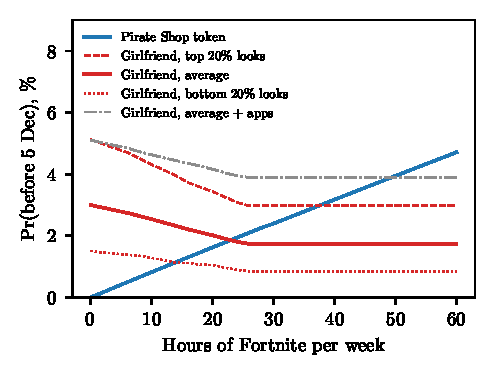
\includegraphics[width=0.5\textwidth]{fig_season.pdf}
\caption{Chance of each before 5 December by hours of Fortnite per week, for solo players who are looking and not on apps. Red lines show the bottom 20\%, average and top 20\% by looks; grey adds dating apps.}
\label{fig:season}
\end{figure}

\paragraph{Your odds.} People often quote a 1\% chance of getting a girlfriend, but that figure is dragged down by the half of single men who are not trying. Effort is the one thing you can change before Christmas, and it beats height comfortably (Table~\ref{tab:effort}).

\begin{table}[!htbp]
\centering\small
\caption{Chance of a girlfriend by Christmas (10 h/week, no apps, average height). Bottom and top are the 10th and 90th percentiles for looks and personality.}
\label{tab:effort}
\begin{tabular}{lrrr}
\toprule
Effort & Bottom & Average & Top \\
\midrule
Not looking & 0.2\% & 0.7\% & 2.4\% \\
Casually looking & 1.0\% & 3.5\% & 11.7\% \\
Actively trying & 2.6\% & 8.5\% & 26.7\% \\
Going all out & 5.1\% & 16.3\% & 46.2\% \\
\bottomrule
\end{tabular}
\end{table}

\paragraph{How many people have it?} Epic will not say. Between 4 and 8 November the daily peak of players in a match averaged 4.1 million~\cite{endgame}, highest on the Saturday, as expected for online games~\cite{vihanga}. Peaks are not averages, since play swings with the time of day~\cite{henderson}, so I assume the average is 40 to 70\% of the peak, that 60 to 90\% of it is Battle Royale, and 39 to 60 chests per match-hour. That is about 2 billion chests a day, or roughly \textbf{14{,}000 tokens a day} (90\% range 9{,}600 to 21{,}000). Each find still costs about 2{,}800 hours of someone's match time. Readers can check the chest rate themselves: Epic also published 1 in 127 for a gizmo~\cite{forbes}, so a solo player on 10 hours a week should see two or three a week.

\paragraph{Uncertainty.} Each of the 23 guessed parameters got a range, and I reran everything 400 times with recalibration. The girlfriend won at 10 hours a week in all 400. The crossover is much less certain, anywhere from 17 to over 60 hours a week (90\% interval). According to the Sobol indices, two guesses dominate: chests per match, and how often relationships end. Neither has an obvious figure. One estimate circulating among players puts squads at 35 chests per player per match~\cite{forbes}, against my 4, and if that is anywhere close then every token number improves several-fold. As for breakups, the literature mostly studies what predicts one rather than how often one happens~\cite{le2010}.

\paragraph{Strategy.} For the completely unemployed and desperate, here is my strategy for the best chance at both. Ten hours a week means about 48 trips to the lobby. Send one DM from each instead of three a week (presuming you have game and the number of girls available to DM doesn't become a limiting factor), and an average casual man goes from 3.5\% to 9\% by Christmas. Add the 5:49 rule and the same ten hours fit 53 matches, which lifts the token to 1.1\% (2.7\% in a squad that leaves together). So, for the best chance of at least one of them: drop with a squad, loot, all die or leave together at 5:49, and DM someone from the bus. This assumes the reply rate stays at 8\% when the messages are coming from a loading screen. If you manage all this, you deserve some luck. You will still need it.

\section{Predictions}

Written on 10 November, to be checked on 5 December.
\begin{enumerate}[noitemsep,topsep=2pt]
\item About 2 in 100 solo players with 100 hours this season will have one (5 in 100 in squads).
\item More than 95\% of 80-hour grinders still won't.
\end{enumerate}

\section{Limitations and Conclusion}

Epic does not publish chests per match or queue times, so I had to estimate these. The dating data describe young American men in general, and if I'm being honest, Fortnite players probably do worse (including me). The height effect is measured on first messages, not relationships. And nothing here shows that Fortnite makes you single. It could potentially run the other way.

So, token or girlfriend? For anyone who is actually looking, the girlfriend, by a distance. Height helps a little. Effort helps a lot. Fortnite skill hardly matters, provided you survive at least the first 2 minutes. A cold DM is 40 times better odds than a chest, and almost nobody sends one, so if you are truly desperate, that's the way to go (although I wouldn't recommend it).

\begin{multicols}{2}

\begin{thebibliography}{99}
\scriptsize\setlength{\itemsep}{0pt}
\bibitem{status} Fortnite Status (@FortniteStatus). Treasure drop rates. Post on X, November 2026.
\bibitem{vgc} Video Games Chronicle. ``Fortnite officially confirms Pirate Shop Access Token drop rate.'' November 2026.
\bibitem{timesaver} FRVR. ``Fortnite Pirate Shop token drop rate explained, and it isn't 1 in 700,000.'' November 2026.
\bibitem{gamesradar} GamesRadar+. ``The Fortnite pirate shop token explained.'' 5 November 2026.
\bibitem{forbes} Tassi, P. ``Fortnite reveals Pirate Shop token drop rates, and they are bad.'' \textit{Forbes}, 8 November 2026.
\bibitem{dexerto} Dexerto. ``YouTuber Typical Gamer misses ultra-rare Fortnite reward by quitting match as a joke in 80-hour grind.'' 9 November 2026.
\bibitem{endgame} Endgame Tools. ``Fortnite player count'' (daily in-match peaks from Epic's data API). Accessed 10 November 2026.
\bibitem{backus} Backus, P. ``Why I don't have a girlfriend: An application of the Drake Equation to love in the UK.'' University of Warwick, 2010.
\bibitem{mortensen} Mortensen, D.\,T. ``Matching: Finding a partner for life or otherwise.'' \textit{American Journal of Sociology} 94:S215--S240, 1988.
\bibitem{charnov} Charnov, E.\,L. ``Optimal foraging, the marginal value theorem.'' \textit{Theoretical Population Biology} 9(2):129--136, 1976.
\bibitem{rosenbusch} Rosenbusch, H. et al. ``Would Chuck Norris certainly win the Hunger Games? Simulating the result reliability of battle royale games through agent-based models.'' \textit{Simulation \& Gaming}, 2020.
\bibitem{sapienza} Sapienza, A. et al. ``Individual performance in team-based online games.'' \textit{Royal Society Open Science} 5(6):180329, 2018.
\bibitem{pew23} Pew Research Center. ``For Valentine's Day, 5 facts about single Americans.'' 2023.
\bibitem{pewod} Pew Research Center. ``Key findings about online dating in the U.S.'' 2023.
\bibitem{atus} U.S. Bureau of Labor Statistics. \textit{American Time Use Survey: 2025 Results}. 2026.
\bibitem{okc} Rudder, C. ``Your looks and your inbox.'' OkCupid blog, 2009.
\bibitem{tyson} Tyson, G. et al. ``A first look at user activity on Tinder.'' \textit{ASONAM}, 2016.
\bibitem{hcmst} Rosenfeld, M.\,J., Thomas, R.\,J. and Hausen, S. ``Disintermediating your friends.'' \textit{PNAS} 116(36):17753--17758, 2019.
\bibitem{nhanes} National Center for Health Statistics. ``Anthropometric reference data for children and adults: United States, August 2021--August 2023.'' \textit{Vital and Health Statistics} 3(50), 2025.
\bibitem{hitsch} Hitsch, G.\,J., Horta\c{c}su, A. and Ariely, D. ``What makes you click? Mate preferences and matching outcomes in online dating.'' MIT Sloan Working Paper 4603-06, 2006.
\bibitem{hensley} Hensley, W.\,E. ``Height as a basis for interpersonal attraction.'' \textit{Adolescence} 29(114), 469--474, 1994.
\bibitem{witmer} Witmer, J. et al. ``The relative importance of looks, height, job, bio, intelligence, and homophily in online dating: A conjoint analysis.'' \textit{Computers in Human Behavior Reports} 17, 100579, 2025.
\bibitem{vihanga} Vihanga, D. et al. ``Weekly seasonal player population patterns in online games.'' \textit{IEEE Conference on Games}, 2019.
\bibitem{henderson} Henderson, T. and Bhatti, S. ``Modelling user behaviour in networked games.'' \textit{ACM Multimedia}, 2001.
\bibitem{larche} Larche, C.\,J. et al. ``Rare loot box rewards trigger larger arousal and reward responses, and greater urge to open more loot boxes.'' \textit{Journal of Gambling Studies}, 2019.
\bibitem{wen} Wen, J.-H. et al. ``Folk models of loot boxes in video games.'' \textit{Proceedings of the ACM on Human-Computer Interaction}, 2024.
\bibitem{xiao} Xiao, L.\,Y. et al. ``Opening Pandora's loot box: Weak links between gambling and loot box expenditure in China, and player opinions on probability disclosures and pity-timers.'' \textit{Journal of Gambling Studies}, 2023.
\bibitem{cordes} Cordes, S. et al. ``What drives demand for loot boxes? An experimental study.'' SSRN working paper, 2024.
\bibitem{bruch} Bruch, E.\,E. and Newman, M.\,E.\,J. ``Aspirational pursuit of mates in online dating markets.'' \textit{Science Advances}, 2018.
\bibitem{kowert} Kowert, R. et al. ``Social gaming, lonely life? The impact of digital game play on adolescents' social circles.'' \textit{Computers in Human Behavior}, 2014.
\bibitem{domahidi} Domahidi, E. et al. ``A longitudinal analysis of gaming- and non-gaming-related friendships and social support among social online game players.'' \textit{Media Psychology}, 2018.
\bibitem{chow} Chow, Y.-S. et al. ``Optimal selection based on relative rank (the `secretary problem').'' \textit{Israel Journal of Mathematics}, 1964.
\bibitem{eriksson} Eriksson, K. et al. ``Optimal stopping in a two-sided secretary problem.'' arXiv, 2004.
\bibitem{saravanakumar} Saravanakumar, P. et al. ``Differential patch-leaving behavior during probabilistic foraging in humans and gerbils.'' \textit{Communications Biology}, 2024.
\bibitem{le2010} Le, B. et al. ``Predicting nonmarital romantic relationship dissolution: A meta-analytic synthesis.'' \textit{Personal Relationships}, 2010.
\bibitem{toma} Toma, C.\,L. et al. ``Separating fact from fiction: An examination of deceptive self-presentation in online dating profiles.'' \textit{Personality and Social Psychology Bulletin}, 2008.
\end{thebibliography}
\end{multicols}

\end{document}
